%% This is file `sample-sigconf.tex',
%% generated with the docstrip utility.
%%
%% The original source files were:
%%
%% samples.dtx  (with options: `sigconf')
% TODO: Change to review before submitting
\documentclass[sigconf]{acmart}
%% \BibTeX command to typeset BibTeX logo in the docs
\AtBeginDocument{%
  \providecommand\BibTeX{{%
    \normalfont B\kern-0.5em{\scshape i\kern-0.25em b}\kern-0.8em\TeX}}}

%% Rights management information.  This information is sent to you
%% when you complete the rights form.  These commands have SAMPLE
%% values in them; it is your responsibility as an author to replace
%% the commands and values with those provided to you when you
%% complete the rights form.
\setcopyright{acmcopyright}
\copyrightyear{2024}
\acmYear{2024}
\acmDOI{XXXXXXX.XXXXXXX}

\acmConference[ICSE 2024]{46th International Conference on Software Engineering}{April 2024}{Lisbon, Portugal}

% My packages
\usepackage[nameinlink]{cleveref} % Reference footnotes.
% My packages end

%%
%% end of the preamble, start of the body of the document source.
\begin{document}

%%
%% The "title" command has an optional parameter,
%% allowing the author to define a "short title" to be used in page headers.
\title{Implementing the Visual Debugger: An Experience report}

\author{Tim Kr\"{a}uter}
\email{tkra@hvl.no}
\orcid{0000-0003-1795-0611}
\affiliation{%
  \institution{Western Norway University of Applied Sciences}
  \city{Bergen}
  \country{Norway}
}

\author{Adrian Rutle}
\email{aru@hvl.no}
\orcid{0000-0002-4158-1644}
\affiliation{%
  \institution{Western Norway University of Applied Sciences}
  \city{Bergen}
  \country{Norway}
}

\author{Harald K\"{o}nig}
\email{harald.koenig@fhdw.de}
\orcid{0000-0001-6304-6311}
\affiliation{%
  \institution{University of Applied Sciences, FHDW}
  \city{Hannover}
  \country{Germany}}
\affiliation{%
  \institution{Western Norway University of Applied Sciences}
  \city{Bergen}
  \country{Norway}
}

\author{Yngve Lamo}
\email{yla@hvl.no}
\orcid{0000-0001-9196-1779}
\affiliation{%
  \institution{Western Norway University of Applied Sciences}
  \city{Bergen}
  \country{Norway}
}

% \author{Patrick Stünkel \orcidlink{0000-0002-0537-295X}}
% \email{patrick.stuenkel@hvl.no}
% \orcid{0000-0002-0537-295X}
% \affiliation{%
%   \institution{Western Norway University of Applied Sciences}
%   \city{Bergen}
%   \country{Norway}
% }

\renewcommand{\shortauthors}{Kräuter et al.}
\newcommand{\intellij}{IntelliJ IDEA}
% 4 pages + 1 page of references.

%%
%% The abstract is a short summary of the work to be presented in the
%% article.
\begin{abstract}
  TODO: Abstract
A demonstration of the visual debugger is available at \url{https://www.youtube.com/watch?v=lU_OgotweRk}.
\end{abstract}

\keywords{IDE, Plugin, Debugging, Visual Debugging, Experience Report, Software Visualization}

% Fitting topics from the workshop:
% 1. The development of plugins, add-ons, and extensions for IDEs.
% 2. Visualizations in the IDEs.
% 3. Anecdotal experience about why a certain tool or research approach was not implemented on top of the IDE infrastructure but researchers chose alternatives (e.g., a CLI tool), what the blockers were, and how the IDEs can improve to become more convenient for prototyping.

\received{7 December 2023}
% \received[revised]{7 December 2023}
% \received[accepted]{11 January 2024}

\maketitle

\section{Introduction}
% Context about the tool
This paper details the experience gained from implementing the visual debugger \cite{krauterVisualDebuggerTool2022}.
The tool is integrated into \intellij \cite{timkrauterVisualDebuggerIntelliJ2023} but its architecture makes it also easily adoptable for other Integrated Development Environments (IDEs).

% Motivation for this report?
% Roadblocks hampering full IDE integration: Swing, Tradeoff tight integration and reusability
% Open problems due to IDE integration: Performance?

% Paper outline
The remainder of this paper is structured as follows.
We describe the visual debugger tool in detail (\cref{sec:visualDebugger}).
Finally, we discuss related work in \cref{sec:relatedWork} and conclude in \cref{sec:conclusion}.


\section{The Visual Debugger Tool} \label{sec:visualDebugger}

\cite{krauterVisualDebuggerTool2022}

\begin{figure}[ht]
  \centering
  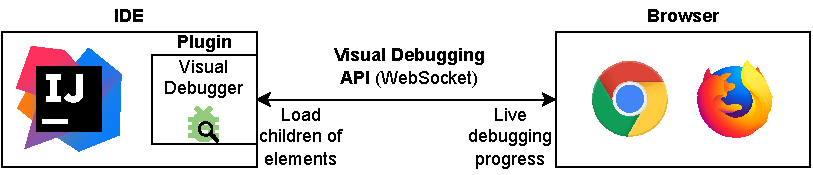
\includegraphics[width=\linewidth]{images/VD-architecture.pdf}
  \caption{Visual Debugger Architecture}
\end{figure}

\section{Lessons Learned: IDE Integration} \label{sec:lessonsLearned}

\section{Related work} \label{sec:relatedWork}

\section{Conclusion} \label{sec:conclusion}

IntelliJ marketplace: \cite{timkrauterVisualDebuggerIntelliJ2023}

Source code: \cite{timkrauterVisualDebuggerTool2023}

Object diagram modeler: \cite{timkrauterObjectDiagramModeler2023}

% \section{Acknowledgments}

\bibliographystyle{ACM-Reference-Format}
\bibliography{bib}
\end{document}
